\documentclass{beamer}
\usetheme{CambridgeUS}
\usecolortheme{default}
\setbeamercolor{itemize item}{fg=darkred!80!black}

\makeatletter
\setbeamertemplate{footline}
{
  \leavevmode%
  \hbox{%
  \begin{beamercolorbox}[wd=.333333\paperwidth,ht=2.25ex,dp=1ex,center]{author in head/foot}%
    \usebeamerfont{author in head/foot}Candidato: F. Massa
  \end{beamercolorbox}%
  \begin{beamercolorbox}[wd=.333333\paperwidth,ht=2.25ex,dp=1ex,center]{title in head/foot}%
    \usebeamerfont{title in head/foot}Relatori: G. Chiarelli, C. Gemme
  \end{beamercolorbox}%
  \begin{beamercolorbox}[wd=.333333\paperwidth,ht=2.25ex,dp=1ex,right]{date in head/foot}%
    \usebeamerfont{date in head/foot}\insertshortdate{}\hspace*{2em}
    \insertframenumber{} / \inserttotalframenumber\hspace*{2ex} 
  \end{beamercolorbox}}%
  \vskip0pt%
}
\makeatother

\title{Tracking Performances of the ATLAS detector \\
for the HL-LHC in the 
$H \rightarrow ZZ^{*} \rightarrow 4\mu$ channel}
%\subtitle{Laurea Magistrale in Fisica}
\author{Federico Massa}
\institute{Laurea Magistrale in Fisica \\
Universit\`a di Pisa}
\date{23 Settembre 2016}

%\setbeameroption{show notes}
\setbeameroption{hide notes}
\setbeamertemplate{navigation symbols}{}

\usepackage{tikz}
\usetikzlibrary{decorations.pathreplacing}
\usetikzlibrary{calc}

\usepackage{amsmath}% mathtools includes this so this is optional
\usepackage{mathtools}

\definecolor{dred}{RGB}{200, 0, 0}

\begin{document}

%-----------------------------------------

\begin{frame}
\titlepage
\end{frame}

\section{Introduzione}

\begin{frame}[t]
\frametitle{Il Large Hadron Collider (LHC)}
\centering
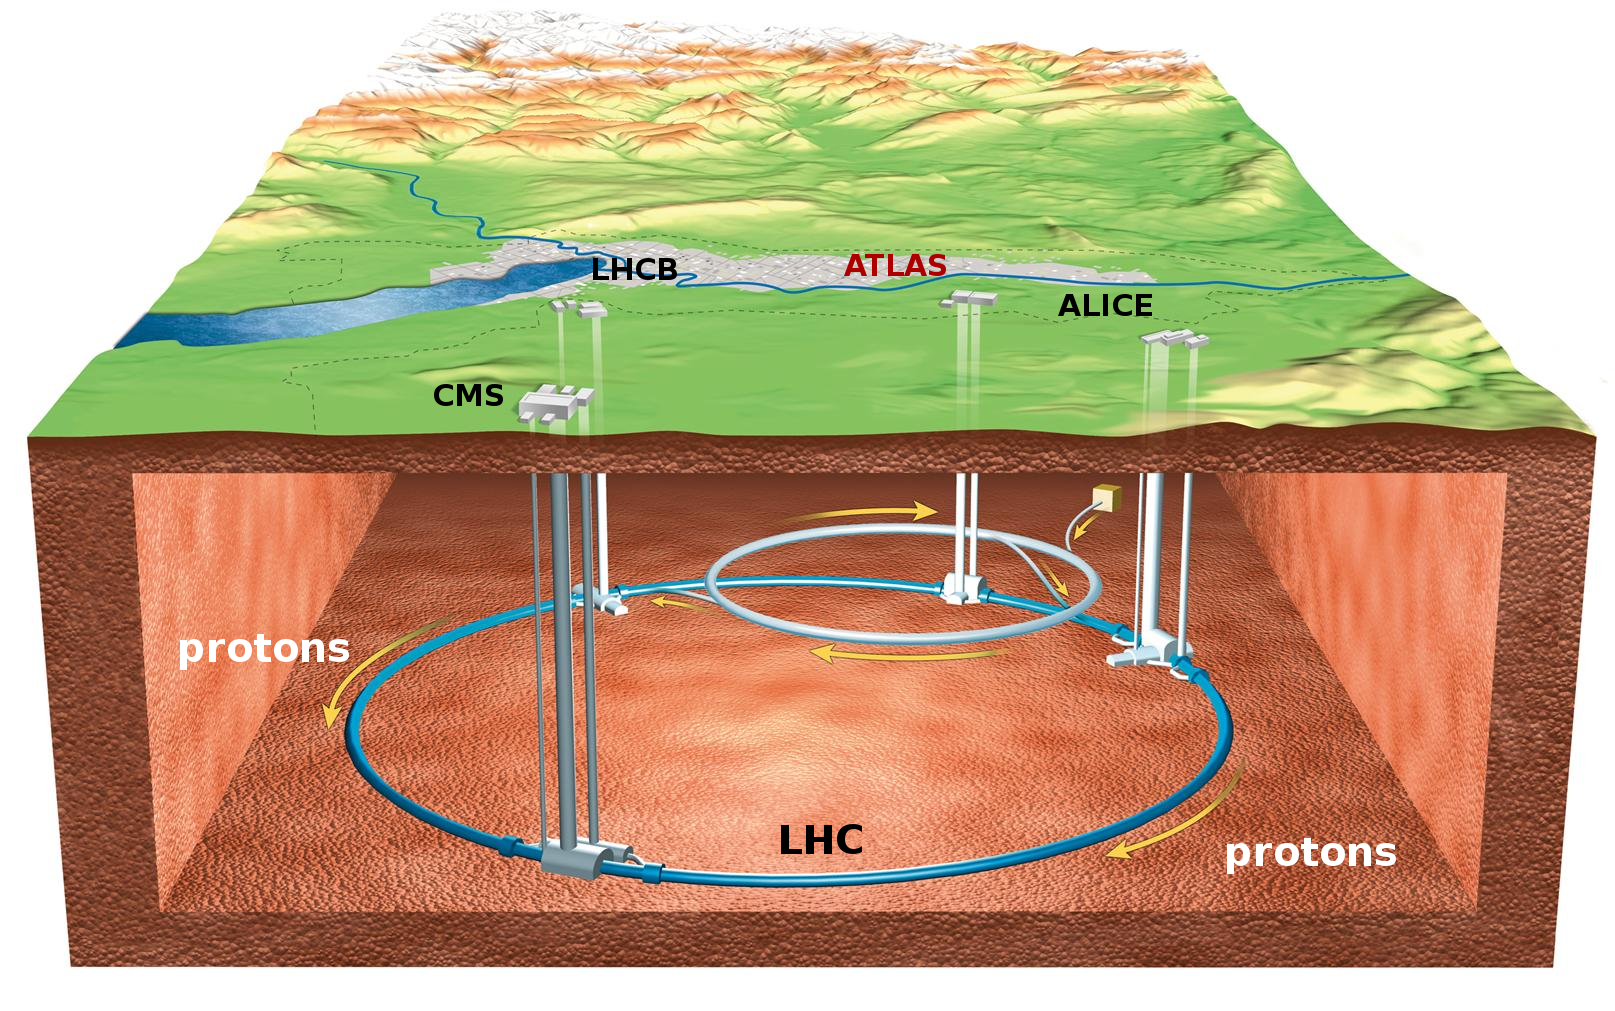
\includegraphics[width=.7\textwidth]{lhc-subterraneo}

\note<1>{
Qui dico che LHC è un sincrotrone che accelera protoni e li fa scontrare
in corrispondenza dei 4 esperimenti, tra i quali ATLAS che è quello di cui
ci siamo occupati. Poi compare l'itemize in cui dico che attualmente sono ad un'energia
di 13 TeV e che ci sono tot bunch ogni 25 ns
}

\onslide<2->{
\begin{itemize}
\item Durante la presa dati attuale (Run 2), i protoni collidono ad un'energia del centro di massa di 13 TeV
\item $\sim$ 2800 ``pacchetti'' (\textit{bunch}) di protoni collidono ogni 25 ns
\end{itemize}}

\end{frame}

%-----------------------------------------

\begin{frame}[t]
\frametitle{Tipi di collisione}
\note<1>{
Abbiamo visto che LHC accelera protoni e fa scontrare i bunch. Cosa succede in una singola
collisione? Pu\`o esserci collisione elastica, pu\`o esserci una collisione inelastica in cui si 
osservano un gran numero di prodotti finali, e ci sono
i processi hard, in cui i quark interagiscono direttamente per dare luogo a interazioni rare ``interessanti''.
}
Le collisioni possono essere:
\begin{itemize}
\item \textbf{elastiche}: i protoni rimangono intatti
\item \textbf{inelastiche}: lo stato finale è diverso da quello iniziale
	\setbeamercolor{local structure}{fg=red}
	\begin{itemize}
	\item \textbf{``hard''}: la collisione avviene direttamente tra partoni con produzione di uno stato finale raro ``interessante'' 
	\end{itemize}
\end{itemize}

\centering
\includegraphics[width=.7\textwidth]{protonCollision}


\end{frame}

%-----------------------------------------

\begin{frame}
\setbeamercolor{normal text}{fg=gray!50!white,bg=}
\setbeamercolor{alerted text}{fg=black,bg=}
\usebeamercolor{normal text}

\frametitle{Il rivelatore di ATLAS}
\begin{columns}
\begin{column}{0.6\textwidth}
\centering
\includegraphics<+->[width=\textwidth]{atlas}
\end{column}
\begin{column}{0.4\textwidth}
	\begin{itemize}
	\item \alert<+>{\small \textbf{Solenoide e toroidi:} producono un campo magnetico che fa curvare
	le particelle cariche}
	\item \alert<+>{\small \textbf{Rivelatore interno:} ricostruisce i vertici e misura l'impulso delle particelle cariche}
	\item \alert<+>{\small \textbf{Calorimetri:} misurano l'energia di particelle cariche e neutre}
	\item \alert<+>{\small \textbf{Camere dei muoni:} misurano l'impulso dei muoni}
	\end{itemize}
\end{column}
\end{columns}
\end{frame}

%-----------------------------------------

\begin{frame}
\frametitle{Il Rivelatore Interno di ATLAS}
\centering

\begin{center}
        \begin{tikzpicture}
            \node[anchor=south west,inner sep=0] (image) at (0,0) {\includegraphics[width=.6\textwidth,angle=-90]{NewID}};
            \node[align=center,red] at ($(image.south east) + (2,1.4)$) {\vbox{\small
            \begin{itemize}
		\item $\eta = -\log{\tan{\frac{\theta}{2}}}$
		\item Copertura angolare: $|\eta| < 2.5$
		\item 4 strati di Pixel
		\item 4 strati di microstrip (SCT) 
		\item Transition Radiation Tracker (TRT)
            \end{itemize}}};
        \end{tikzpicture}
    \end{center}

\end{frame}

%-----------------------------------------

\begin{frame}[t]
\frametitle{Numero di interazioni}

\note<1>{
Definisco R = L$\sigma$  e dico che il numero di interazioni per bunch è dato da N = L$\times \sigma_{inel.} \times 25$ ns
}

Il numero medio di interazioni per unit\`a di tempo \`e dato da\\
\medskip

\begin{columns}
\begin{column}{0.4\textwidth}
$$
\frac{dN}{dt} =\sigma \times \mathcal{L}
$$
\end{column}
\begin{column}{0.6\textwidth}
\end{column}
\end{columns}
\medskip
con:\\
\begin{itemize}
\item $\mathcal{L}$: \textbf{luminosit\`a istantanea}, termine geometrico che descrive la geometria del fascio 
\item $\sigma$: \textbf{sezione d'urto} del processo considerato
\item $\int\mathcal{L}dt$: \textbf{luminosit\`a integrata} nel tempo di presa dati
\end{itemize}
\bigskip 

\onslide<2->{
Il numero medio di interazioni per ``bunch-crossing'' \`e quindi:\\
\begin{columns}
\begin{column}{0.6\textwidth}
$$
\langle\mu\rangle = \sigma_{inel.} \times \mathcal{L} \times 25\ \mathrm{ns} \mathrm{\mathbf{\ \simeq 23\ }(Run 2)} 
$$
\end{column}
\begin{column}{0.4\textwidth}
\end{column}
\end{columns}

}
\end{frame}

%-----------------------------------------

\begin{frame}[t]
\frametitle{High Luminosity LHC (HL-LHC)}
\note<1>{
Sono previsti una serie di upgrade ad LHC, in particolare quello del 2026 che porterà ad HL-LHC, in cui la luminosit\`a 
passer\`a dal valore attuale di $10^{34}$ a 7.5 x $10^{34}$ e prevede di durare 10 anni, raccogliendo 3000 fb$^{-1}$ di dati a 14 TeV.
}

LHC prevede una serie di upgrade per aumentare la luminosit\`a istantanea \\
\ \ \ \ \ \ \ \ \ \ \  $\rightarrow$ \textbf{High-Luminosity LHC} (HL-LHC)
\vskip0.2cm
\includegraphics[width=\textwidth]{HLLHC_Plan}

\begin{columns}
\begin{column}{0.7\textwidth}
\end{column}
\begin{column}{0.3\textwidth}

\begin{tikzpicture}[scale=1]
\draw [decorate,decoration={brace,amplitude=8pt},xshift=-50pt,yshift=0pt, dred, thick]
(3.5,0) -- (0,0); %node [midway,xshift=-0cm]{};
\end{tikzpicture}
\end{column}
\end{columns}
\medskip
\begin{itemize}
\item HL-LHC prevede di raccogliere una luminosit\`a integrata di 3000 fb$^{-1}$
\item Massima luminosit\`a istantanea: 7.5 $\times 10^{34}$ cm$^{-2}$s$^{-1}$
\item L'energia del centro di massa sar\`a quella di progetto: 14 TeV
\end{itemize}

\end{frame}

%-----------------------------------------

\begin{frame}[t]
\frametitle{Pile-up}
Il numero di collisioni per ``bunch-crossing'' ad HL-LHC aumenta
a causa dell'aumento della luminosit\`a e della sezione d'urto inelastica.\\

\begin{itemize}
\item Le collisioni che avvengono \textit{nello stesso bunch} di quella di interesse
rappresentano il cosiddetto \textbf{in-time pile-up}
\item valore nominale ad HL-LHC: 140
\item valore di picco ad HL-LHC: 200
\end{itemize}

\only<1>{\includegraphics[width=\textwidth]{collisions20}}
\only<2>{\includegraphics[width=\textwidth, height=4cm]{collisions140}}



\end{frame}

%-----------------------------------------



%-----------------------------------------

\begin{frame}
\frametitle{Upgrade per HL-LHC}
L'attuale rivelatore interno \`e inadatto alla fase di alta luminosit\`a:
\pause
\begin{itemize}
\item<+-> I rivelatori a pixel e SCT non sono disegnati per sopportare l'alto
flusso di radiazione di HL-LHC
\item<+-> L'elettronica di read-out \`e disegnata per un numero massimo di eventi
		di pile-up di 50 $\rightarrow$ inefficienze ad HL-LHC
\item<+-> La risoluzione spaziale dell'SCT non permette di risolvere tracce
		in ambienti altamente densi di particelle
\item<+-> Il TRT raggiunger\`a il 100\% di occupancy (frazione di canali elettronici attivi)
\end{itemize}

\bigskip

\onslide<+->{\Large{\color{dred}\textbf{\ \ \ $\rightarrow$ Necessario upgrade: Inner Tracker (ITk)}}}

\end{frame}

%-----------------------------------------

\begin{frame}
\frametitle{Layout di ITk: Step-1}


\begin{columns}
\begin{column}{0.5\textwidth}
	\begin{itemize}
	\item Solo rivelatori al silicio \\ (no TRT)
	\item Copertura angolare estesa: $|\eta| < 2.5 \rightarrow 4.0$
	\item 5 strati di pixel + 4 SCT
	\item Pixel a maggiore risoluzione
	\end{itemize}
	\ \ \ \
\end{column}
\begin{column}{0.5\textwidth}
\includegraphics[width=\textwidth,height=3.8cm]{ExtBrl4}
\end{column}
\end{columns}

\begin{columns}
\begin{column}{0.5\textwidth}
\includegraphics[width=\textwidth,height=3.8cm]{IExtBrl4}
\end{column}
\begin{column}{0.5\textwidth}
\includegraphics[width=\textwidth,height=3.8cm]{InclBrl4}
\end{column}
\end{columns}

\end{frame}

%-----------------------------------------



%-----------------------------------------

\end{document}